% Provenance (never printed): see sources/outline_sources.md (Year 1: gravity and its
% measurement, normal gravity; isostasy, Airy and Pratt; free-air and Bouguer anomalies;
% the geoid). Curves from figdata/bachelor-1/hypsometry.py and gravity_profiles.py;
% exercise and problem values in the Book 3 scratch calculator calc/ch11.py.
\chapter{Isostasia e anomalias da gravidade}\label{ch:b1:isostasy-gravity}

Nos anos 1840 os topógrafos que mediam um arco de meridiano pelo norte da Índia
encontraram uma discrepância que não podiam atribuir aos instrumentos. Entre duas estações
a cerca de 370 milhas, Kaliana, ao pé do Himalaia, e Kalianpur, muito mais ao sul, a
diferença de \omterm{def:b1:spherical-astronomy:geographic}{latitude} obtida por triangulação excedeu a obtida pelas estrelas em
5.236 segundos de arco. O culpado óbvio eram as montanhas: sua atração puxa um fio de prumo para o norte, e os
astrônomos ajustavam seus instrumentos pelo fio de prumo. Em 1855 John Henry Pratt
calculou a atração do Himalaia e dos planaltos além dele e
encontrou que ela deveria ter feito a discrepância ser de 15.885 segundos, mais de três
vezes o que foi observado. As montanhas puxavam muito menos do que sua massa visível
exigia. No mesmo ano George Airy respondeu que a \omterm{def:b1:layered-earth:layers}{crosta} flutua sobre uma camada mais densa
como uma jangada de toras sobre a água, de modo que terrenos altos têm uma raiz profunda de
rocha leve; Pratt propôs depois outra resposta, uma rocha tornada mais leve pela
expansão sob as montanhas. As duas ainda são ensinadas: as montanhas têm embaixo rocha leve que compensa
sua massa. Este capítulo transforma essa ideia em
números, e mostra como a gravidade, medida a um milionésimo de seu valor, revela as
massas escondidas sob a topografia.
% ledger: pratt:himalaya, airy:1855, pratt:1871

\begin{recall}
A lei de gravitação de Newton dá o campo $g = GM/r^2$ fora de uma massa esférica
$M$; o campo deriva de um potencial gravitacional, e uma superfície equipotencial é em todo
ponto perpendicular ao campo (física). Em um fluido em repouso a pressão cresce com a profundidade como $\mathrm dp/\mathrm dz = \rho g$, e um
corpo flutuante desloca seu próprio peso de fluido (física, primeiro ano universitário).
Abaixo da \omterm{def:b1:layered-earth:lithosphere}{litosfera} a \omterm{def:b1:layered-earth:lithosphere}{astenosfera} flui ao longo de tempos longos; a \omterm{def:b1:layered-earth:layers}{crosta} é mais leve que o \omterm{def:b1:layered-earth:layers}{manto} embaixo dela (\cref{ch:b1:layered-earth}; Livro 2, 11º ano).
\end{recall}

\section{A gravidade e sua medida}

A aceleração da gravidade na superfície da Terra é próxima de \qty{9.8}{m.s^{-2}}, e as
variações que interessam aos geólogos são um milhão de vezes menores. Elas são contadas em uma
unidade do antigo sistema centímetro--grama, o gal: $\qty{1}{Gal} = \qty{1}{cm.s^{-2}} = \qty{0.01}{m.s^{-2}}$, de modo
que
\[
  \qty{1}{\milli\gal} = \qty{e-5}{m.s^{-2}} \approx \num{e-6}\,g .
\]
% ledger: nist:gal
Um gravímetro de campo resolve alguns milésimos de miligal; as anomalias
estudadas neste capítulo vão de uma fração de miligal sobre um corpo de minério enterrado a
algumas centenas de miligals sobre uma cadeia de montanhas.

Mesmo em uma Terra sem topografia, a gravidade não seria a mesma em toda parte. A Terra gira, de
modo que o que um fio de prumo ou um gravímetro sente é a soma da atração gravitacional e do
efeito centrífugo da rotação; e a Terra é achatada, de modo que os polos ficam mais perto de seu
centro que o equador.
Os dois efeitos tornam a gravidade mais fraca no equador do que nos polos. Um geólogo
compara cada medida com uma referência suave que as contém.

\begin{definition}[Gravidade normal]\label{def:b1:isostasy-gravity:normal-gravity}
A \emph{gravidade normal}\index{gravidade normal} $\gamma$ é a gravidade de um modelo
da Terra: um elipsoide de revolução com a massa e a rotação da Terra, escolhido de modo que
sua superfície seja uma equipotencial de sua própria gravidade (gravitação mais o efeito
centrífugo). Nessa superfície, a gravidade normal depende apenas da \omterm{def:b1:spherical-astronomy:geographic}{latitude}.
\end{definition}

O elipsoide em si, seu achatamento e a maneira como seus parâmetros são ajustados à
Terra real são estudados no Livro 5. Aqui precisamos apenas de sua gravidade.

\begin{proposition}[A fórmula da gravidade normal]\label{prop:b1:isostasy-gravity:normal-formula}
No elipsoide de referência adotado em 1980, a \omterm{def:b1:isostasy-gravity:normal-gravity}{gravidade normal} na \omterm{def:b1:spherical-astronomy:geographic}{latitude} geográfica
$\varphi$ é, em sua forma usual em série,
\[
  \gamma(\varphi) = \qty{9.780327}{m.s^{-2}}\,\bigl(1 + 0.0053024\sin^2\varphi
  - 0.0000058\sin^2 2\varphi\bigr).
\]
\end{proposition}
\admitted
% ledger: moritz:grs80

Ela dá \qty{9.780327}{m.s^{-2}} no equador, \qty{9.806200}{m.s^{-2}} a
\ang{45} e \qty{9.832186}{m.s^{-2}} nos polos: uma diferença de
\qty{5186}{\milli\gal} do equador ao polo. A rotação sozinha explica
a maior parte. Com o dia sideral de \qty{23.9345}{h}, a velocidade angular é
$\omega = 2\pi/\qty{86164}{s} = \qty{7.292e-5}{rad.s^{-1}}$, e a aceleração centrífuga
no equador, $\omega^2 a$ com $a = \qty{6378.137}{km}$, é
\qty{0.0339}{m.s^{-2}}, ou \qty{3392}{\milli\gal}; o achatamento fornece o
resto (\cref{exo:b1:isostasy-gravity:2}).
% ledger: earth:Trot, earth:Req, earth:geq, earth:gpole

A gravidade é medida de duas maneiras. Um gravímetro \emph{absoluto} deixa cair uma massa de teste
em uma câmara de vácuo e acompanha sua queda livre com um interferômetro a laser,
cronometrado por um relógio atômico: a aceleração sai diretamente da distância e do
tempo. Um gravímetro \emph{relativo} é uma massa pendurada em uma mola, cujo alongamento
muda com a gravidade; é leve e rápido, mas só dá diferenças entre lugares, e deriva,
de modo que um levantamento retorna a uma estação-base cuja gravidade é conhecida. Os
melhores instrumentos absolutos têm precisão de cerca de um microgal, uma parte em um bilhão de
$g$.
% ledger: ngs:absolute-gravity

\begin{inthefield}[Um levantamento gravimétrico em terra]
\begin{minipage}[t]{0.55\linewidth}\vspace{0pt}
Um levantamento gravimétrico é uma caminhada lenta de estação em estação. Em cada uma, o geofísico
instala o gravímetro relativo no seu tripé, nivela-o, espera a mola se acomodar e faz várias leituras; um
receptor de posicionamento por satélite ao lado registra a posição e a altura da estação. A cada poucas horas
a equipe volta à estação-base, para que a deriva da mola possa ser medida e removida. A altura importa tanto quanto a gravidade: como mostra a próxima seção, a gravidade cai
\qty{0.3086}{\milli\gal} para cada metro de altura, de modo que uma altura errada em \qty{1}{cm} estraga a leitura em
\qty{3}{\micro\gal}. % ledger: usgs73:reduction
\end{minipage}\hfill
\begin{minipage}[t]{0.42\linewidth}\vspace{0pt}
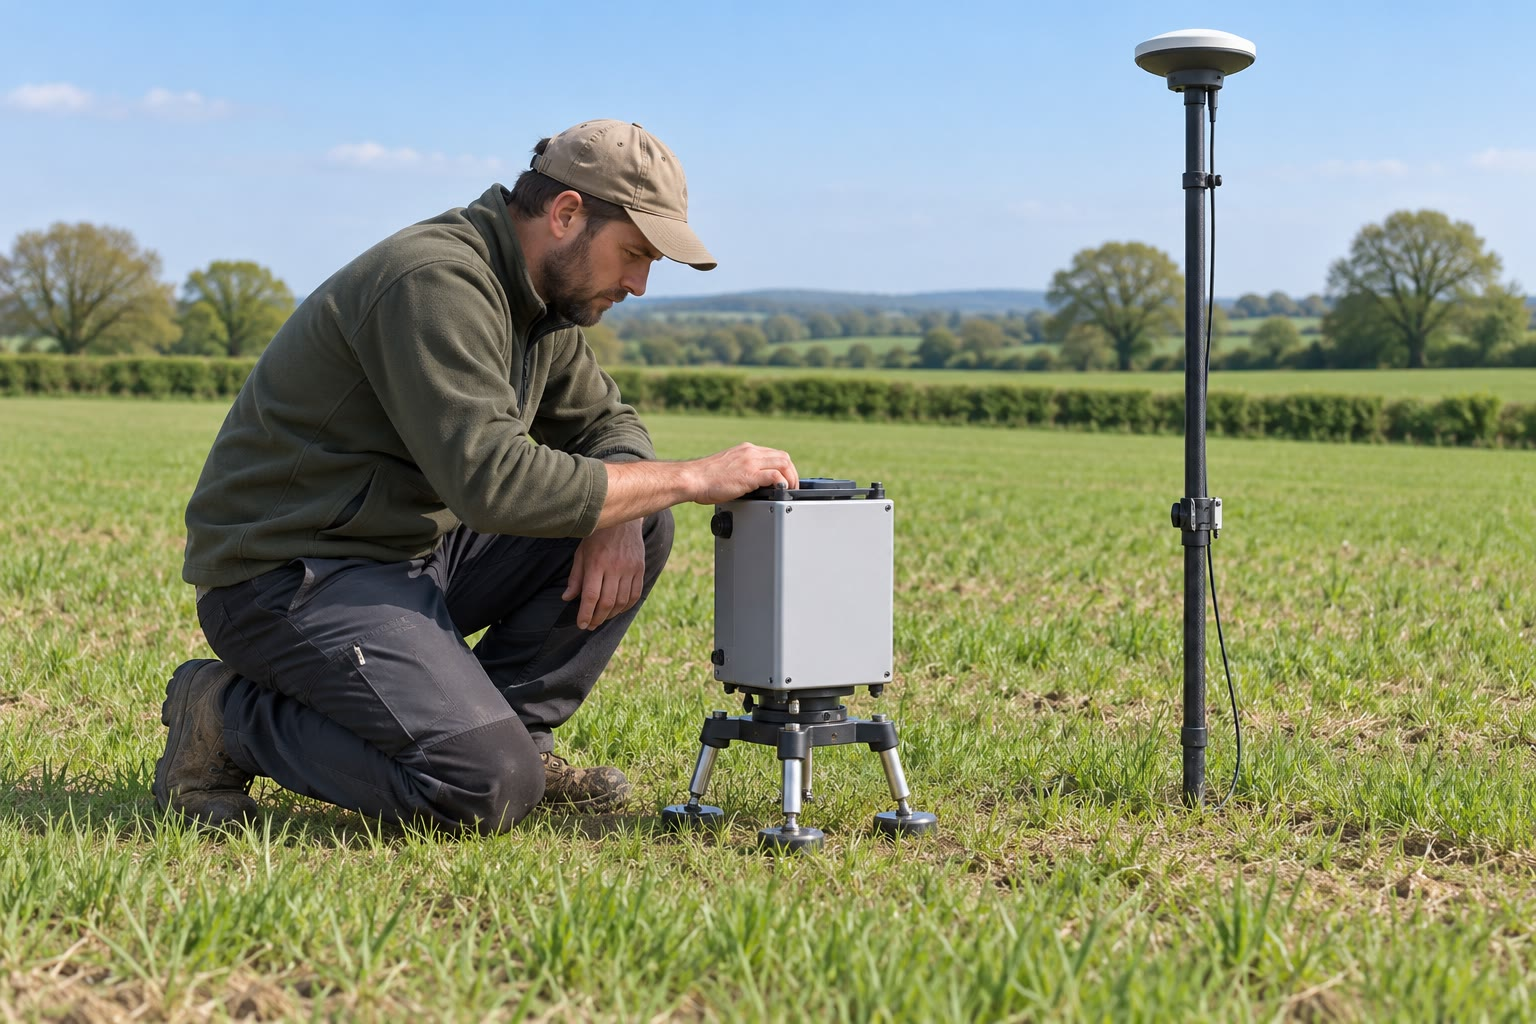
\includegraphics[width=\linewidth]{images/book3/ai/b1-gravity-survey.jpg}

{\scriptsize Um gravímetro de campo sobre seu tripé, com uma antena de posicionamento por satélite ao lado (ilustração gerada por IA).}
\end{minipage}
\end{inthefield}

\section{Isostasia}

A compensação imaginada por Airy e Pratt para o Himalaia é um caso de um
estado geral das camadas externas da Terra.

\begin{definition}[Isostasia; profundidade de compensação]\label{def:b1:isostasy-gravity:isostasy}
Uma região está em \emph{isostasia}\index{isostasia}, ou equilíbrio isostático, quando
existe uma profundidade, a \emph{profundidade de compensação}\index{profundidade de compensação},
na qual a pressão é a mesma em todo ponto da superfície horizontal, qualquer que seja a topografia
acima dela. Abaixo da profundidade de compensação as rochas se comportam como um fluido em repouso;
acima dela, as colunas de \omterm{def:b1:layered-earth:layers}{crosta} e \omterm{def:b1:layered-earth:layers}{manto} flutuam sobre elas.
\end{definition}

\begin{proposition}[Massas iguais acima da profundidade de compensação]\label{prop:b1:isostasy-gravity:equal-mass}
Se a gravidade $g$ é a mesma ao longo de todas as colunas, uma região está em \omterm{def:b1:isostasy-gravity:isostasy}{isostasia} com
\omterm{def:b1:isostasy-gravity:isostasy}{profundidade de compensação} $z_c$ se, e somente se, toda coluna vertical de seção unitária,
da superfície até $z_c$, contém a mesma massa.
\end{proposition}

\begin{proof}
Em cada coluna as rochas estão em equilíbrio hidrostático, de modo que
$\mathrm dp/\mathrm dz = \rho(z)\,g$, com a profundidade $z$ contada para baixo. A
pressão na superfície é atmosférica, a mesma em toda parte (e desprezível).
Integrando desde a superfície $z_s$ da coluna até $z_c$ obtém-se
\[
  p(z_c) = p_0 + g\int_{z_s}^{z_c}\rho(z)\,\mathrm dz ,
\]
em que a integral é a massa da coluna por unidade de área. As pressões em
$z_c$ são iguais se, e somente se, essas massas o forem.
\end{proof}

Duas maneiras simples de distribuir as massas dão os dois modelos clássicos
(figura abaixo).

\begin{proposition}[Isostasia de Airy]\label{prop:b1:isostasy-gravity:airy}
Seja a \omterm{def:b1:layered-earth:layers}{crosta} de densidade uniforme $\rho_c$ e espessura $H$ onde sua
superfície está ao nível do mar, sobre um \omterm{def:b1:layered-earth:layers}{manto} de densidade $\rho_m > \rho_c$. Em equilíbrio
isostático:
\begin{enumerate}
  \item onde a superfície está a uma altura $h$ acima do nível do mar, a \omterm{def:b1:layered-earth:layers}{crosta} tem
        uma raiz de profundidade $r = h\,\rho_c/(\rho_m - \rho_c)$ abaixo da \omterm{def:b1:layered-earth:layers}{crosta} normal,
        e uma espessura $H + h + r$;
  \item onde a superfície está a uma profundidade $d$ abaixo do nível do mar, sob água de
        densidade $\rho_w$, a \omterm{def:b1:layered-earth:layers}{crosta} tem uma anti-raiz: sua base é elevada em
        $r' = d\,(\rho_c - \rho_w)/(\rho_m - \rho_c)$, e sua espessura é
        $H - d - r'$.
\end{enumerate}
Isto é a \emph{isostasia de Airy}\index{isostasia de Airy}: compensação por variações de
espessura, com densidade constante.
\end{proposition}

\begin{proof}
Tome a \omterm{def:b1:isostasy-gravity:isostasy}{profundidade de compensação} logo abaixo da raiz mais profunda, e compare cada
coluna com a normal. (1) A coluna alta tem \omterm{def:b1:layered-earth:layers}{crosta} no lugar do \omterm{def:b1:layered-earth:layers}{manto}
ao longo da profundidade $r$, e \omterm{def:b1:layered-earth:layers}{crosta} ao longo da altura $h$ onde a coluna normal não tem
nada: massas iguais exigem $\rho_c(h + r) = \rho_m r$, isto é
$r(\rho_m - \rho_c) = \rho_c h$. (2) A coluna baixa tem água no lugar da \omterm{def:b1:layered-earth:layers}{crosta}
ao longo da profundidade $d$, e \omterm{def:b1:layered-earth:layers}{manto} no lugar da \omterm{def:b1:layered-earth:layers}{crosta} ao longo de $r'$: massas iguais exigem
$\rho_w d + \rho_m r' = \rho_c(d + r')$, isto é $r'(\rho_m - \rho_c) =
d(\rho_c - \rho_w)$.
\end{proof}

\begin{proposition}[Isostasia de Pratt]\label{prop:b1:isostasy-gravity:pratt}
Seja cada coluna terminando na mesma \omterm{def:b1:isostasy-gravity:isostasy}{profundidade de compensação} $D$ abaixo do nível do mar, com uma
densidade uniforme em cada coluna, $\rho_0$ onde a superfície está ao nível do mar. Em
equilíbrio isostático, uma coluna cuja superfície está a uma altura $h$ tem a
densidade
\[
  \rho(h) = \rho_0\,\frac{D}{D + h},
\]
e uma coluna sob uma profundidade $d$ de água tem a densidade
$\rho = (\rho_0 D - \rho_w d)/(D - d)$. Isto é a \emph{isostasia de Pratt}\index{isostasia de Pratt}: compensação por variações de densidade a
profundidade constante.
\end{proposition}

\begin{proof}
Massas iguais acima de $D$: $\rho(h)(D + h) = \rho_0 D$ para a coluna alta, e
$\rho_w d + \rho(D - d) = \rho_0 D$ para a baixa.
\end{proof}

Com $\rho_c = \qty{2700}{kg.m^{-3}}$ e $\rho_m = \qty{3300}{kg.m^{-3}}$, a raiz de Airy é
$h\times2700/600 = 4.5\,h$: uma cordilheira de \qty{2}{km} de altura tem uma raiz de
\qty{9}{km}, um planalto de \qty{4}{km} de altura uma de \qty{18}{km}. No modelo de Pratt
com $D = \qty{100}{km}$ e $\rho_0 = \qty{2700}{kg.m^{-3}}$, as mesmas duas
colunas têm as densidades 2647 e \qty{2596}{kg.m^{-3}}, duas e quatro por cento
mais leves. Os dois modelos equilibram as mesmas massas; diferem no lugar da rocha leve,
e isso é algo que a sismologia pode ver: Airy prevê um \omterm{def:b1:layered-earth:discontinuity}{Moho} que se aprofunda sob as montanhas,
Pratt um \omterm{def:b1:layered-earth:discontinuity}{Moho} plano.

\begin{omfigure}
\begin{tikzpicture}[x=0.55cm, y=0.05cm, font=\scriptsize]
% columns computed in calc/ch11.py: Airy roots 9 and 18 km, Pratt densities 2647 and 2596 kg/m3;
% heights above sea level drawn five times larger than depths
\begin{scope}
  \node[font=\small] at (4.5,30) {(a) Airy};
  \fill[omLithGranite!45] (0,0) rectangle (3,-35);
  \fill[omLithGranite!45] (3,10) rectangle (6,-44);
  \fill[omLithGranite!45] (6,20) rectangle (9,-53);
  \fill[omLithPeridotite!45] (0,-35) rectangle (3,-60);
  \fill[omLithPeridotite!45] (3,-44) rectangle (6,-60);
  \fill[omLithPeridotite!45] (6,-53) rectangle (9,-60);
  \draw (0,-60) -- (0,0) -- (3,0) -- (3,10) -- (6,10) -- (6,20) -- (9,20) -- (9,-60);
  \draw (3,0) -- (3,-60) (6,10) -- (6,-60);
  \draw[thick] (0,-35) -- (3,-35) -- (3,-44) -- (6,-44) -- (6,-53) -- (9,-53);
  \draw[densely dashed] (-0.3,-60) -- (9.3,-60);
  \draw[black!50, densely dotted] (-0.3,0) -- (0,0);
  \node[anchor=east] at (-0.3,0) {nível do mar};
  \node[anchor=east] at (-0.3,-35) {35};
  \node[anchor=east] at (-0.3,-60) {60 km};
  \node at (1.5,-17) {2700}; \node at (4.5,-20) {2700}; \node at (7.5,-24) {2700};
  \node at (1.5,-50) {3300};
  \node[anchor=south] at (1.5,0) {$h = 0$};
  \node[anchor=south] at (4.5,10) {$h = 2$};
  \node[anchor=south] at (7.5,20) {$h = 4$};
  \draw[black!45, densely dotted] (3,-35) -- (9,-35);
  \node at (4.5,-39.5) {raiz 9};
  \node at (7.5,-44) {raiz 18};
\end{scope}
\begin{scope}[xshift=7.9cm]
  \node[font=\small] at (4.5,30) {(b) Pratt};
  \fill[omLithGranite!45] (0,0) rectangle (3,-100);
  \fill[omLithGranite!36] (3,10) rectangle (6,-100);
  \fill[omLithGranite!27] (6,20) rectangle (9,-100);
  \draw (0,-100) -- (0,0) -- (3,0) -- (3,10) -- (6,10) -- (6,20) -- (9,20) -- (9,-100);
  \draw (3,0) -- (3,-100) (6,10) -- (6,-100);
  \draw[densely dashed] (-0.3,-100) -- (9.3,-100);
  \draw[black!50, densely dotted] (-0.3,0) -- (0,0);
  \node[anchor=east] at (-0.3,0) {nível do mar};
  \node[anchor=east] at (-0.3,-100) {$D = 100$ km};
  \node at (1.5,-50) {2700}; \node at (4.5,-50) {2647}; \node at (7.5,-50) {2596};
  \node[anchor=south] at (1.5,0) {$h = 0$};
  \node[anchor=south] at (4.5,10) {$h = 2$};
  \node[anchor=south] at (7.5,20) {$h = 4$};
\end{scope}
\end{tikzpicture}

\par\smallskip{\small Os dois modelos clássicos de \omterm{def:b1:isostasy-gravity:isostasy}{isostasia}, para três colunas
de altura 0, 2 e \qty{4}{km} acima do nível do mar (alturas exageradas cinco vezes
em relação às profundidades; densidades em \unit{kg.m^{-3}}). (a) Airy: uma densidade crustal,
uma raiz 4.5 vezes a altura. (b) Pratt: uma \omterm{def:b1:isostasy-gravity:isostasy}{profundidade de compensação}, colunas mais leves
sob terrenos mais altos. Cada coluna carrega a mesma massa por unidade de área acima da
\omterm{def:b1:isostasy-gravity:isostasy}{profundidade de compensação} tracejada.}
\label{fig:b1:isostasy-gravity:models}
\end{omfigure}

A \omterm{def:b1:isostasy-gravity:isostasy}{isostasia} é uma afirmação sobre regiões amplas em tempos longos. A \omterm{def:b1:layered-earth:lithosphere}{astenosfera} cede
apenas a cargas que persistem por milhares de anos, e a \omterm{def:b1:layered-earth:lithosphere}{litosfera} acima dela é rígida o bastante para espalhar uma carga estreita por uma região ampla, por flexão,
como uma tábua que sustenta um peso: um único vulcão não precisa ser compensado embaixo de
si mesmo; essa flexão da \omterm{def:b1:layered-earth:lithosphere}{litosfera} é estudada no Livro 5. Sob grandes cadeias de montanhas a \omterm{def:b1:layered-earth:layers}{crosta} é muito mais espessa que sua média continental, de cerca de
\qty{30}{km}: a imagem de Airy, raízes de \omterm{def:b1:layered-earth:layers}{crosta} leve, é a mais próxima para cadeias de montanhas. A de Pratt, rocha mais leve a profundidade constante, explica as
dorsais meso-oceânicas, que ficam altas sobre um \omterm{def:b1:layered-earth:layers}{manto} superior tornado mais leve pela
sua temperatura mais alta.
% ledger: usgs:crust-thickness

\subsection*{Os dois níveis da Terra}

A \omterm{def:b1:isostasy-gravity:isostasy}{isostasia} organiza a topografia do planeta inteiro. Sua distribuição é
resumida por uma curva.

\begin{definition}[Curva hipsométrica]\label{def:b1:isostasy-gravity:hypsometry}
A \emph{curva hipsométrica}\index{curva hipsométrica} de um planeta dá, para
cada fração $f$ de sua superfície, a altitude $z(f)$ ultrapassada exatamente por essa
fração. É a distribuição acumulada das altitudes, lida de cima.
\end{definition}

Para desenhá-la a partir de um modelo de elevação em grade, cada célula da grade deve ser ponderada por
sua área. Em uma grade de um grau em \omterm{def:b1:spherical-astronomy:geographic}{latitude} e \omterm{def:b1:spherical-astronomy:geographic}{longitude}, a célula entre
as \omterm{def:b1:spherical-astronomy:geographic}{latitudes} $\varphi_1$ e $\varphi_2$ tem a área
$R^2\,\Delta\lambda\,(\sin\varphi_2 - \sin\varphi_1)$, que diminui em direção aos
polos; somadas todas as células, as áreas dão $4\pi R^2$ exatamente. Ordenando as
células por altitude e acumulando suas áreas obtém-se a curva da figura
abaixo. Ela mostra que \qty{70.9}{\percent} da superfície fica abaixo do nível do mar;
que a altitude média das terras é cerca de \qty{0.8}{km} e a profundidade média do
oceano cerca de \qty{3.7}{km}; e que a maior parte da superfície pertence a um de
dois degraus planos, as plataformas continentais perto do nível do mar e o fundo abissal
entre cerca de 3.5 e \qty{6}{km} de profundidade, unidos por uma queda abrupta.
% computed in figdata/bachelor-1/hypsometry.py (fraction 0.709, land 793 m, ocean 3692 m); ledger: data:etopo1, wss:ocean-cover

Um planeta com um único tipo de \omterm{def:b1:layered-earth:layers}{crosta}, com sua topografia erguida e desgastada ao acaso,
teria um só nível, com altitudes espalhadas em torno dele. A Terra tem dois,
porque tem dois tipos de \omterm{def:b1:layered-earth:layers}{crosta} em equilíbrio isostático: a \omterm{def:b1:layered-earth:layers}{crosta} continental, espessa e leve,
flutua alta; a \omterm{def:b1:layered-earth:layers}{crosta} oceânica, fina e densa, fica baixa (Livro 2, 11º ano).
\Cref{exo:b1:isostasy-gravity:8} mostra que o modelo de Airy, com uma só densidade crustal,
não consegue produzir os dois níveis com as espessuras crustais observadas.

\begin{omfigure}
\begin{tikzpicture}
\begin{axis}[omrecord, width=0.84\linewidth, height=6.4cm, xmin=0, xmax=100, ymin=-11, ymax=9,
  xlabel={fração da superfície da Terra situada mais alto (\unit{\percent})},
  ylabel={altitude (km)}, xtick={0,10,...,100}, ytick={-10,-8,...,8},
  tick label style={font=\scriptsize}, label style={font=\small}, clip=true]
% computed in figdata/bachelor-1/hypsometry.py; ledger: data:etopo1
\addplot[name path=hyps, very thick, black] table[x=area_pc, y expr=\thisrow{elev}/1000] {figdata/out/bachelor-1-hypsometry-curve.dat};
\path[name path=sea] (axis cs:0,0) -- (axis cs:100,0);
\addplot[omSea!60] fill between[of=hyps and sea, soft clip={domain=29.1:100}];
\addplot[omHypsLandC!80] fill between[of=hyps and sea, soft clip={domain=0:29.1}];
\draw[black!60, densely dotted] (axis cs:0,0) -- (axis cs:100,0);
\draw[black!60, densely dashed] (axis cs:29.1,-11) -- (axis cs:29.1,9);
\draw[omSea!60!black, densely dashed] (axis cs:29.1,-3.692) -- (axis cs:100,-3.692);
\draw[omHypsLandF, densely dashed] (axis cs:0,0.793) -- (axis cs:29.1,0.793);
\node[font=\scriptsize, anchor=south east] at (axis cs:99,0.1) {nível do mar};
\node[font=\scriptsize, anchor=south, align=center] at (axis cs:18,1.0) {altitude média\\das terras \qty{0.79}{km}};
\node[font=\scriptsize, anchor=north west, align=left] at (axis cs:31,-3.9) {profundidade média\\do oceano \qty{3.69}{km}};
\node[font=\scriptsize, anchor=north west, align=left] at (axis cs:30.5,6.5) {terras: \qty{29.1}{\percent}\\da superfície};
\node[font=\scriptsize, anchor=north, align=center] at (axis cs:17,-0.5) {plataforma\\continental};
\node[font=\scriptsize] at (axis cs:62,-5.2) {fundo abissal};
\end{axis}
\end{tikzpicture}

\par\smallskip{\small A \omterm{def:b1:isostasy-gravity:hypsometry}{curva hipsométrica} da Terra, a partir do modelo global de topografia ETOPO1 a um grau, com cada célula ponderada por sua área (sobre a Antártida e a
Groenlândia, o topo do gelo). Os dois trechos quase planos da curva são as plataformas continentais
perto do nível do mar e o fundo oceânico profundo.}
\label{fig:b1:isostasy-gravity:hypsometry}
\end{omfigure}

\section{Anomalias da gravidade}

\subsection*{Duas correções}

Um gravímetro numa colina está mais longe do centro da Terra que um ao nível do mar,
e fica sobre uma camada de rocha que o outro não tem. Os dois efeitos são
calculados antes de a medida ser comparada com a \omterm{def:b1:isostasy-gravity:normal-gravity}{gravidade normal}.

\begin{proposition}[Gradiente do ar livre]\label{prop:b1:isostasy-gravity:free-air}
Fora de uma Terra esférica de raio $R$, a gravidade diminui com a altura $h$ à
taxa
\[
  \frac{\mathrm dg}{\mathrm dh} = -\frac{2g}{R}\,;
\]
na superfície, $2g/R \approx \qty{3.08e-6}{s^{-2}}$, cerca de
\qty{0.308}{\milli\gal} por metro.
\end{proposition}

\begin{proof}
$g(r) = GM/r^2$, logo $\mathrm dg/\mathrm dr = -2GM/r^3 = -2g(r)/r$; em $r = R$,
com $g = \qty{9.820}{m.s^{-2}}$ e $R = \qty{6371}{km}$, $2g/R =
\qty{3.083e-6}{s^{-2}}$.
\end{proof}
% ledger: earth:gmean, earth:Rmean

O achatamento e a rotação alteram um pouco o gradiente; o valor normalmente usado na
prática é \qty{0.3086}{\milli\gal.m^{-1}}.
% ledger: usgs73:reduction

\begin{proposition}[Placa de Bouguer]\label{prop:b1:isostasy-gravity:slab}
Uma placa horizontal infinita de espessura $h$ e densidade uniforme $\rho$ atrai
um ponto fora dela com a aceleração vertical
\[
  g_B = 2\pi G\rho h ,
\]
qualquer que seja a distância do ponto à placa. Numericamente $2\pi G =
\qty{0.0419}{\milli\gal}$ por metro de espessura por \qty{1000}{kg.m^{-3}} de
densidade.
\end{proposition}

\begin{proof}
Coloque o ponto na origem e corte a placa em anéis finos coaxiais com a
vertical que passa por ele. Um anel à distância $z$ abaixo do ponto, de raio
$s$, largura $\mathrm ds$ e espessura $\mathrm dz$, tem a massa
$\rho\,2\pi s\,\mathrm ds\,\mathrm dz$, toda à distância $\sqrt{s^2 + z^2}$;
por simetria sua atração é vertical, igual à atração de cada
elemento vezes o cosseno $z/\sqrt{s^2+z^2}$ de seu ângulo com a vertical:
\[
  \mathrm dg = G\,\frac{\rho\,2\pi s\,\mathrm ds\,\mathrm dz}{s^2 + z^2}\,
  \frac{z}{\sqrt{s^2 + z^2}} .
\]
Para uma camada, $\int_0^\infty s\,(s^2 + z^2)^{-3/2}\,\mathrm ds =
\bigl[-(s^2 + z^2)^{-1/2}\bigr]_0^\infty = 1/z$, logo a camada atrai com
$2\pi G\rho\,\mathrm dz$, independentemente de $z$. Somando as camadas ao longo da
espessura $h$ dá $2\pi G\rho h$. Com $G = \qty{6.674e-11}{m^3.kg^{-1}.s^{-2}}$,
$2\pi G\times\qty{1000}{kg.m^{-3}}\times\qty{1}{m} = \qty{4.19e-7}{m.s^{-2}} =
\qty{0.0419}{\milli\gal}$.
\end{proof}
% ledger: const:G

\begin{definition}[Anomalias da gravidade]\label{def:b1:isostasy-gravity:anomalies}
Seja $g$ a gravidade medida em uma estação de \omterm{def:b1:spherical-astronomy:geographic}{latitude} $\varphi$ e altura $h$
acima do nível do mar.
\begin{itemize}
  \item Uma \emph{anomalia da gravidade}\index{anomalia da gravidade} é a diferença
        entre a gravidade medida, corrigida a um nível comum, e a
        \omterm{def:b1:isostasy-gravity:normal-gravity}{gravidade normal} na mesma \omterm{def:b1:spherical-astronomy:geographic}{latitude}.
  \item A \emph{correção do ar livre}\index{correção do ar livre} é
        $+\qty{0.3086}{\milli\gal.m^{-1}}\times h$: ela devolve a diminuição
        da gravidade com a altura. A \emph{anomalia do ar
        livre}\index{anomalia do ar livre} é
        $\Delta g_{\mathrm{FA}} = g + 0.3086\,h - \gamma(\varphi)$.
  \item A \emph{correção de Bouguer}\index{correção de Bouguer} é $-2\pi G\rho h$:
        ela remove a atração da rocha entre a estação e o nível do mar, tratada como uma placa de
        densidade $\rho$, convencionalmente \qty{2670}{kg.m^{-3}}, o que dá \qty{0.112}{\milli\gal} por metro.
        A \emph{anomalia de Bouguer}\index{anomalia de Bouguer} é
        $\Delta g_{\mathrm B} = \Delta g_{\mathrm{FA}} - 2\pi G\rho h$.
\end{itemize}
\end{definition}
% ledger: usgs73:reduction, swisstopo:bouguer-map

A placa é um modelo grosseiro do terreno em torno de uma estação em região acidentada: vales abaixo
da estação são contados como rocha que não está lá, e colinas acima dela puxam para cima e não são contadas de modo algum.
Uma terceira redução, a correção de terreno, calculada a partir de um \omterm{def:b1:geological-maps:dem}{modelo digital de elevação}, remove os dois erros.
No mar a \omterm{def:b1:isostasy-gravity:anomalies}{correção do ar livre} se anula, e a redução de Bouguer substitui a água por rocha.

\begin{method}[Redução de uma leitura gravimétrica]\label{met:b1:isostasy-gravity:reduction}
\begin{enumerate}
  \item Calcule a \omterm{def:b1:isostasy-gravity:normal-gravity}{gravidade normal} $\gamma(\varphi)$ na \omterm{def:b1:spherical-astronomy:geographic}{latitude} da estação.
  \item Some a \omterm{def:b1:isostasy-gravity:anomalies}{correção do ar livre} $0.3086\,h$ (em \unit{\milli\gal}, com $h$
        em metros) à gravidade medida e subtraia $\gamma$: esta é a
        \omterm{def:b1:isostasy-gravity:anomalies}{anomalia do ar livre}.
  \item Subtraia a \omterm{def:b1:isostasy-gravity:anomalies}{correção de Bouguer} $0.0419\times(\rho/1000)\times h$, isto é
        $0.112\,h$ para a densidade padrão: esta é a \omterm{def:b1:isostasy-gravity:anomalies}{anomalia de Bouguer}.
  \item Trabalhe em miligals do início ao fim, e mantenha a gravidade medida e a normal
        com sete algarismos significativos: a anomalia é uma pequena diferença de dois
        números grandes.
\end{enumerate}
\end{method}

\begin{example}[Uma estação nas colinas]\label{ex:b1:isostasy-gravity:reduction}
Em uma estação a \omterm{def:b1:spherical-astronomy:geographic}{latitude} \ang{45} e \qty{1200}{m} acima do nível do mar, o gravímetro dá \qty{9.802597}{m.s^{-2}}. A \omterm{def:b1:isostasy-gravity:normal-gravity}{gravidade normal} ali é
\qty{9.806200}{m.s^{-2}}; o valor medido é menor em \qty{360.3}{\milli\gal}.
A \omterm{def:b1:isostasy-gravity:anomalies}{correção do ar livre} é $0.3086\times1200 = \qty{370.3}{\milli\gal}$, logo
$\Delta g_{\mathrm{FA}} = -360.3 + 370.3 = \qty{+10.0}{\milli\gal}$. A \omterm{def:b1:isostasy-gravity:anomalies}{correção de
Bouguer} é $0.112\times1200 = \qty{134.4}{\milli\gal}$, logo $\Delta g_{\mathrm B}
= \qty{-124.4}{\milli\gal}$: há menos massa sob esta estação do que sob uma
estação ao nível do mar, depois que a rocha acima do nível do mar é retirada.
\end{example}

\subsection*{O que as anomalias dizem sobre a compensação}

\begin{proposition}[Anomalias sobre uma topografia ampla]\label{prop:b1:isostasy-gravity:broad}
Considere um planalto de altura $h$ e densidade $\rho_c$, muito mais largo que sua
\omterm{def:b1:isostasy-gravity:isostasy}{profundidade de compensação}, e uma estação perto de seu centro. Tome a densidade de Bouguer
igual a $\rho_c$.
\begin{enumerate}
  \item Se o planalto não está compensado, $\Delta g_{\mathrm{FA}} \approx
        2\pi G\rho_c h$ e $\Delta g_{\mathrm B} \approx 0$.
  \item Se ele está em equilíbrio isostático, qualquer que seja a distribuição das
        massas de compensação, $\Delta g_{\mathrm{FA}} \approx 0$ e
        $\Delta g_{\mathrm B} \approx -2\pi G\rho_c h$.
\end{enumerate}
\end{proposition}

\begin{proof}
A \omterm{def:b1:isostasy-gravity:normal-gravity}{gravidade normal} à altura da estação é $\gamma - 0.3086\,h$, logo a \omterm{def:b1:isostasy-gravity:anomalies}{anomalia do ar
livre} é a atração das massas que diferem das de uma
coluna normal. Perto do centro de um planalto amplo, cada camada dessas massas anômalas
atua como uma placa infinita, e, pela \cref{prop:b1:isostasy-gravity:slab}, uma placa de
contraste de densidade $\Delta\rho$ e espessura $t$ atrai com $2\pi G\Delta\rho
t$ onde quer que esteja. O total é $2\pi G$ vezes a massa anômala por unidade de
área. (1) Sem compensação essa massa é $\rho_c h$. (2) Em \omterm{def:b1:isostasy-gravity:isostasy}{isostasia} ela é
nula, pela \cref{prop:b1:isostasy-gravity:equal-mass}. Nos dois casos a \omterm{def:b1:isostasy-gravity:anomalies}{correção de Bouguer}
subtrai $2\pi G\rho_c h$.
\end{proof}

Para a compensação de Airy, a \omterm{def:b1:isostasy-gravity:anomalies}{anomalia de Bouguer} do segundo caso é também
$-2\pi G(\rho_m - \rho_c)r$, a atração da massa ausente da raiz,
pois $(\rho_m - \rho_c)r = \rho_c h$. \omterm{def:b1:isostasy-gravity:anomalies}{Anomalias do ar livre} próximas de zero sobre regiões amplas
são portanto a assinatura da \omterm{def:b1:isostasy-gravity:isostasy}{isostasia}, e \omterm{def:b1:isostasy-gravity:anomalies}{anomalias de Bouguer} que seguem
a topografia como imagem especular medem as massas de compensação: as \omterm{def:b1:isostasy-gravity:anomalies}{anomalias de Bouguer}
são regionalmente negativas ao longo dos Alpes, e sobre as dorsais meso-oceânicas,
por mais altas que sejam, a \omterm{def:b1:isostasy-gravity:anomalies}{anomalia do ar livre} é pequena. Sobre os oceanos a
\omterm{def:b1:isostasy-gravity:anomalies}{anomalia de Bouguer} é positiva: substituir a água por rocha acrescenta massa acima de uma
coluna que não tem massa ausente.
% ledger: swisstopo:bouguer-map

Perto das bordas da topografia a aproximação de placa falha, porque a topografia está próxima da estação e a raiz muito abaixo dela. A figura abaixo
dá a atração exata de uma cadeia-modelo de \qty{200}{km} de largura e \qty{2}{km}
de altura. Sem compensação, a \omterm{def:b1:isostasy-gravity:anomalies}{anomalia do ar livre} é
\qty{+225}{\milli\gal} no centro, próxima do valor da placa de
\qty{226}{\milli\gal}; com uma raiz de Airy de \qty{9}{km}, a \omterm{def:b1:isostasy-gravity:anomalies}{anomalia do ar livre} no centro
cai para \qty{+55}{\milli\gal}, e não zero, porque uma cadeia com apenas
\qty{200}{km} de largura não parece infinita a \qty{40}{km} acima de sua raiz, e
a \omterm{def:b1:isostasy-gravity:anomalies}{anomalia do ar livre} torna-se fortemente negativa logo além de cada borda, onde a
estação vê a raiz, mas não a montanha.
% computed in figdata/bachelor-1/gravity_profiles.py (centre values 225.0, -1.4, 55.2, -171.2 mGal)

\begin{omfigure}
\begin{tikzpicture}
\begin{axis}[omrecord, name=anom, width=0.86\linewidth, height=6.2cm, xmin=-300, xmax=300, ymin=-310, ymax=250,
  ylabel={anomalia (\unit{\milli\gal})}, xticklabels={}, ytick={-200,-100,0,100,200},
  tick label style={font=\scriptsize}, label style={font=\small},
  legend style={font=\scriptsize, at={(0.01,0.01)}, anchor=south west, draw=none, fill=white, fill opacity=0.85, text opacity=1},
  legend cell align=left, legend columns=2]
% computed in figdata/bachelor-1/gravity_profiles.py
\addplot[very thick, red!75!black] table[x=x, y=fa_unc] {figdata/out/bachelor-1-gravity_profiles-profiles.dat};
\addlegendentry{ar livre, sem compensação}
\addplot[thick, red!75!black, densely dashed] table[x=x, y=bg_unc] {figdata/out/bachelor-1-gravity_profiles-profiles.dat};
\addlegendentry{Bouguer, sem compensação}
\addplot[very thick, blue!70!black] table[x=x, y=fa_airy] {figdata/out/bachelor-1-gravity_profiles-profiles.dat};
\addlegendentry{ar livre, raiz de Airy}
\addplot[thick, blue!70!black, densely dashed] table[x=x, y=bg_airy] {figdata/out/bachelor-1-gravity_profiles-profiles.dat};
\addlegendentry{Bouguer, raiz de Airy}
\draw[black!50, densely dotted] (axis cs:-300,0) -- (axis cs:300,0);
\end{axis}
\begin{axis}[at={(anom.south west)}, anchor=north west, yshift=-0.25cm, width=0.86\linewidth, height=3.6cm,
  xmin=-300, xmax=300, ymin=-50, ymax=5, axis background/.style={fill=white},
  xlabel={distância do centro da cadeia (km)}, ylabel={profundidade (km)},
  ytick={0,-35,-44}, yticklabels={0,35,44}, tick label style={font=\scriptsize}, label style={font=\small}]
\fill[omLithPeridotite!45] (axis cs:-300,-50) rectangle (axis cs:300,-35);
\fill[omLithGranite!45] (axis cs:-300,-35) rectangle (axis cs:300,0);
\fill[omLithGranite!45] (axis cs:-100,0) rectangle (axis cs:100,2);
\fill[omLithGranite!45, pattern color=blue!60!black, postaction={pattern=north east lines, pattern color=blue!50!black}] (axis cs:-100,-35) rectangle (axis cs:100,-44);
\draw (axis cs:-300,0) -- (axis cs:-100,0) -- (axis cs:-100,2) -- (axis cs:100,2) -- (axis cs:100,0) -- (axis cs:300,0);
\draw[thick] (axis cs:-300,-35) -- (axis cs:300,-35);
\draw[thick, blue!60!black] (axis cs:-100,-35) -- (axis cs:-100,-44) -- (axis cs:100,-44) -- (axis cs:100,-35);
\node[font=\scriptsize] at (axis cs:-200,-17) {crosta 2700};
\node[font=\scriptsize] at (axis cs:-200,-43) {manto 3300};
\node[font=\scriptsize, fill=white, inner sep=1pt, anchor=west] at (axis cs:105,-40) {raiz de Airy (segundo modelo)};
\node[font=\scriptsize, anchor=south] at (axis cs:0,2) {cadeia, \qty{2}{km} de altura};
\end{axis}
\end{tikzpicture}

\par\smallskip{\small Acima: \omterm{def:b1:isostasy-gravity:anomalies}{anomalias do ar livre} e de Bouguer através de uma cadeia-modelo
de \qty{200}{km} de largura e \qty{2}{km} de altura, calculadas exatamente para corpos bidimensionais, com estações sobre a superfície do terreno (sem correção de terreno).
Abaixo: o modelo (escala vertical exagerada menos de duas vezes); a raiz existe apenas no caso
compensado. Sem compensação, a \omterm{def:b1:isostasy-gravity:anomalies}{anomalia do ar livre} segue a topografia e a \omterm{def:b1:isostasy-gravity:anomalies}{anomalia de Bouguer} é quase nula;
compensada, a \omterm{def:b1:isostasy-gravity:anomalies}{anomalia do ar livre} é pequena no centro, com efeitos de borda agudos, e a \omterm{def:b1:isostasy-gravity:anomalies}{anomalia de Bouguer} é um vale amplo.}
\label{fig:b1:isostasy-gravity:profiles}
\end{omfigure}

\begin{method}[Teste de isostasia para uma região]\label{met:b1:isostasy-gravity:test}
\begin{enumerate}
  \item Calcule a média da \omterm{def:b1:isostasy-gravity:anomalies}{anomalia do ar livre} sobre uma área várias vezes mais larga que a
        espessura da \omterm{def:b1:layered-earth:layers}{crosta}, longe das bordas da topografia.
  \item Se estiver perto de zero, a região está compensada; se se aproximar de
        $2\pi G\rho_c$ vezes a altura média, não está.
  \item A razão $-\Delta g_{\mathrm B}/(2\pi G\rho_c h)$ dá a fração da topografia que está compensada.
  \item Evidências sísmicas ou de outro tipo sobre a profundidade do \omterm{def:b1:layered-earth:discontinuity}{Moho} distinguem a
        compensação de Airy da de Pratt: a gravidade em grande escala sozinha não consegue, pois as duas colocam
        o mesmo déficit de massa sob a topografia.
\end{enumerate}
\end{method}

\begin{history}[A gravidade no mar]
\begin{minipage}[t]{0.58\linewidth}\vspace{0pt}
Um pêndulo mede a gravidade pelo seu período, mas em um navio as ondas o sacodem muito mais do que qualquer anomalia. Nos anos 1920 o geodesista holandês Felix Vening
Meinesz achou o caminho: dois pêndulos oscilando em fase oposta no mesmo quadro sentem as mesmas acelerações horizontais do navio, e sua diferença as cancela. A partir de 1923 ele levou seu aparelho em submarinos da marinha holandesa, onde, submersos, era poupado do pior das ondas, primeiro em uma viagem às Índias Orientais e depois em levantamentos de seus mares.
Ao longo das fossas oceânicas profundas do arquipélago encontrou longas faixas de anomalias isostáticas fortemente negativas, e depois as encontrou ao longo de outras fossas: só podia explicá-las por uma \omterm{def:b1:layered-earth:layers}{crosta} mantida para baixo ali por forças externas, fora do equilíbrio isostático.
% ledger: egs:vening-meinesz
\end{minipage}\hfill
\begin{minipage}[t]{0.38\linewidth}\vspace{0pt}
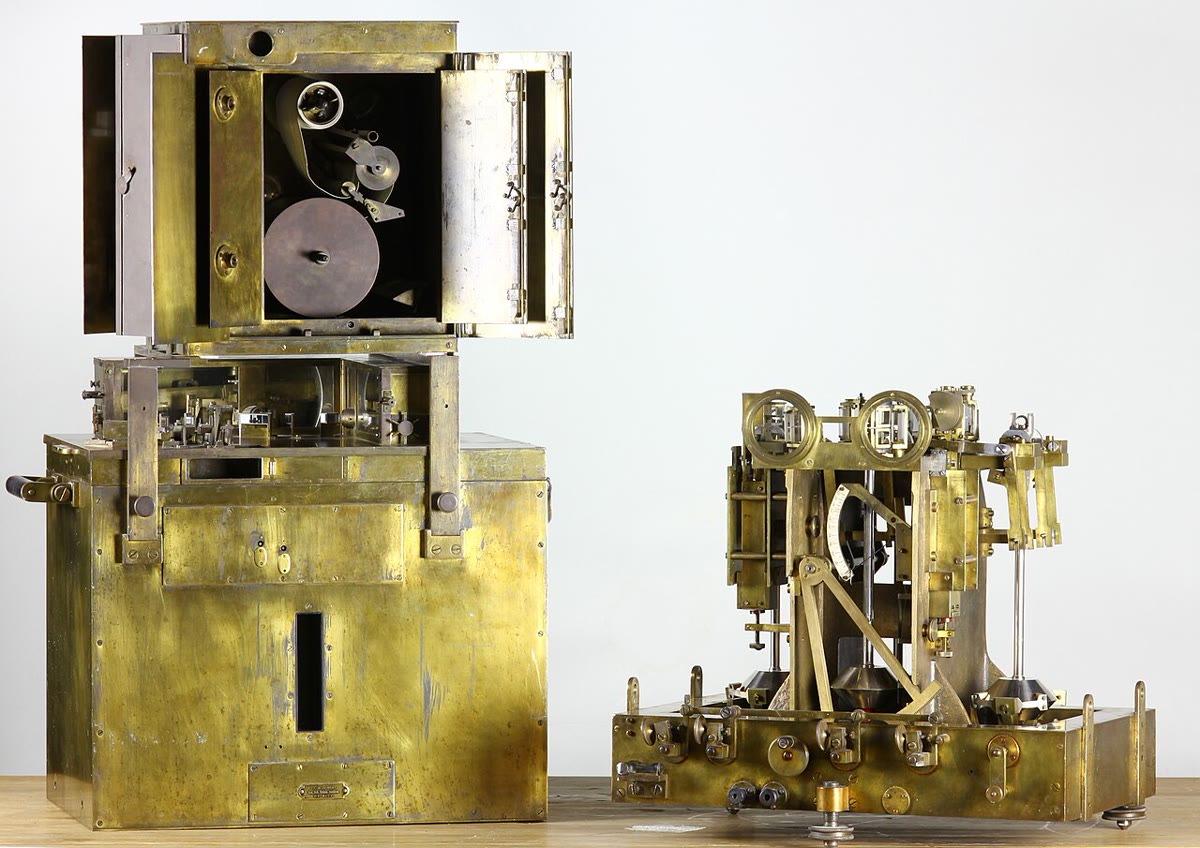
\includegraphics[width=\linewidth]{images/book3/b1-vening-meinesz.jpg}

{\scriptsize Um aparelho de pêndulo de Vening Meinesz (à direita) e sua caixa com a
unidade de registro (Broodt, CC BY-SA 4.0).}
\end{minipage}
\end{history}

\section{O geoide}

A superfície do mar em repouso é uma superfície de potencial gravitacional constante: se não fosse,
a água fluiria ao longo dela. É a referência natural para as alturas, e
a superfície à qual os antigos fios de prumo eram perpendiculares.

\begin{definition}[Geoide; altura do geoide]\label{def:b1:isostasy-gravity:geoid}
O \emph{geoide}\index{geoide} é a superfície equipotencial da gravidade da Terra (gravitação mais o efeito centrífugo da rotação) que coincide
com a superfície média do mar sobre os oceanos abertos, em repouso, e se prolonga sob os continentes. A \emph{altura do geoide}\index{altura do geoide} $N$ em um
ponto é a altura do geoide acima do elipsoide de referência, contada negativa onde o geoide fica abaixo dele.
\end{definition}

As alturas acima do nível do mar nos mapas são alturas acima do \omterm{def:b1:isostasy-gravity:geoid}{geoide}; as alturas dadas pelo posicionamento por satélite são alturas acima do elipsoide; as duas diferem por
$N$. O \omterm{def:b1:isostasy-gravity:geoid}{geoide} se afasta do elipsoide em \qty{+85}{m} perto da Islândia e \qty{-106}{m} ao largo do sul da Índia, menos de \qty{200}{m} no total, enquanto a topografia
da superfície sólida abrange cerca de \qty{20}{km}: o \omterm{def:b1:isostasy-gravity:geoid}{geoide} é uma superfície muito mais suave que o terreno.
% ledger: nasa:geoid-range, earth:topo

\begin{proposition}[Altura do geoide e anomalia do potencial]\label{prop:b1:isostasy-gravity:bruns}
Seja $\Phi$ o potencial gravitacional da Terra e $\Phi_n$ o potencial normal,
o da Terra-modelo cuja superfície, o elipsoide de referência, tem o mesmo
potencial $\Phi_0$ que o \omterm{def:b1:isostasy-gravity:geoid}{geoide}, ambos contados com o sinal da física (o
potencial cresce para cima e $g = -\nabla\Phi$). Seja $T = \Phi - \Phi_n$ a
anomalia do potencial no \omterm{def:b1:isostasy-gravity:geoid}{geoide}. Em primeira ordem,
\[
  N = -\frac{T}{\gamma} .
\]
Os geodesistas, que contam o potencial com o sinal oposto, escrevem o mesmo
resultado $N = T/\gamma$, a fórmula de Bruns.
\end{proposition}

\begin{proof}
Seja $Q$ um ponto do elipsoide e $P$ o ponto do \omterm{def:b1:isostasy-gravity:geoid}{geoide} sobre a
normal por $Q$, à altura $N$. O potencial normal cresce para cima
à taxa $\gamma$, logo $\Phi_n(P) \approx \Phi_n(Q) + \gamma N = \Phi_0 +
\gamma N$. Como $P$ está no \omterm{def:b1:isostasy-gravity:geoid}{geoide}, $\Phi(P) = \Phi_0$, isto é
$\Phi_n(P) + T = \Phi_0$. Logo $\Phi_0 + \gamma N + T = \Phi_0$ e $N =
-T/\gamma$.
\end{proof}

Um excesso de massa abaixo de um ponto torna ali o potencial mais negativo, logo
$T < 0$ e $N > 0$: o \omterm{def:b1:isostasy-gravity:geoid}{geoide} se eleva sobre um excesso de massa e afunda sobre um
déficit. Os \qty{85}{m} da elevação perto da Islândia correspondem a uma anomalia de potencial
de $-\qty{85}{m}\times\qty{9.8}{m.s^{-2}} \approx \qty{-830}{J.kg^{-1}}$.
Como o potencial decai como $1/r$ enquanto a atração decai como $1/r^2$,
o \omterm{def:b1:isostasy-gravity:geoid}{geoide} é dominado por massas grandes e profundas, e as \omterm{def:b1:isostasy-gravity:anomalies}{anomalias da gravidade} por
massas rasas. Uma cadeia de montanhas compensada eleva o \omterm{def:b1:isostasy-gravity:geoid}{geoide} apenas pouco,
pois seu excesso de massa e o déficit de sua raiz quase se cancelam; uma
carga não compensada o eleva muito mais.

\begin{omfigure}
\begin{tikzpicture}[x=1.15cm, y=1.3cm, font=\scriptsize, >={Stealth[length=4pt]}]
% schematic, not to scale
\fill[omSea!35] (0,0.05) .. controls (1.5,0.25) and (2.5,0.35) .. (3.6,0.45) -- (3.6,-1.2) -- (0,-1.2) -- cycle;
\fill[omLithGranite!40] (3.6,0.45) .. controls (4.5,1.4) and (5.4,1.9) .. (6.4,1.7) .. controls (7.4,1.5) and (8.2,1.2) .. (9,1.0) -- (9,-1.2) -- (3.6,-1.2) -- cycle;
\fill[omLithGabbro!35] (0,-0.7) .. controls (1.2,-0.9) and (2.4,-0.6) .. (3.6,-0.2) -- (3.6,-1.2) -- (0,-1.2) -- cycle;
\draw[thick, blue!70!black] (0,0.05) .. controls (1.5,0.25) and (2.5,0.35) .. (3.6,0.45) .. controls (5,0.75) and (7,0.75) .. (9,0.55);
\draw[thick, black, densely dashed] (0,-0.25) .. controls (3,0.05) and (6,0.15) .. (9,0.1);
\draw (3.6,0.45) .. controls (4.5,1.4) and (5.4,1.9) .. (6.4,1.7) .. controls (7.4,1.5) and (8.2,1.2) .. (9,1.0);
\node[anchor=west, blue!70!black] at (9.05,0.6) {geoide};
\node[anchor=west] at (9.05,0.1) {elipsoide};
\node[anchor=west] at (9.05,1.0) {terreno};
\node at (1.4,-0.3) {oceano};
\node at (1.6,-1.0) {fundo do mar};
% heights (curve ordinates computed from the Bezier segments)
\draw[<->] (6.6,0.107) -- (6.6,0.688); \node[anchor=east] at (6.57,0.40) {$N$};
\draw[<->] (7.2,0.674) -- (7.2,1.512); \node[anchor=west] at (7.23,1.09) {$H$};
\draw[<->] (8.2,0.110) -- (8.2,1.224); \node[anchor=east] at (8.17,0.95) {$h_e$};
% the vertical (perpendicular to the geoid) and the ellipsoid normal at x = 2.4 (angle exaggerated)
\draw[->, thick, blue!70!black] (2.4,0.335) -- (2.0,1.3);
\draw[->, thick, black] (2.4,0.335) -- (2.33,1.3);
\node[anchor=south east, blue!70!black] at (2.05,1.3) {vertical (fio de prumo)};
\node[anchor=south west] at (2.3,1.3) {normal ao elipsoide};
\end{tikzpicture}

\par\smallskip{\small O \omterm{def:b1:isostasy-gravity:geoid}{geoide} (azul), o elipsoide de referência (tracejado) e o
terreno (esquemático; desvios enormemente exagerados). Sobre o oceano o \omterm{def:b1:isostasy-gravity:geoid}{geoide} é a superfície do mar em repouso; sob a terra ele se prolonga como uma equipotencial.
A altura $H$ em um mapa é medida a partir do \omterm{def:b1:isostasy-gravity:geoid}{geoide}, a altura $h_e$ dada pelo posicionamento por satélite a partir do elipsoide, e $h_e = H + N$. Um fio de prumo é
perpendicular ao \omterm{def:b1:isostasy-gravity:geoid}{geoide}, não ao elipsoide: o ângulo entre eles (exagerado aqui) é o desvio da vertical que preocupou os topógrafos da Índia.}
\label{fig:b1:isostasy-gravity:geoid}
\end{omfigure}

Os desvios são pequenos: toda a discrepância que preocupou os topógrafos
da Índia foi de cerca de cinco segundos de arco. Sobre os oceanos o \omterm{def:b1:isostasy-gravity:geoid}{geoide} é visível.
Desde 1978, altímetros de radar em satélites cronometram pulsos de micro-ondas
refletidos pela superfície do mar para medir sua altura. Uma vez eliminadas marés, ondas e
correntes por média, a superfície do mar fica mais alta sobre montes submarinos e
dorsais e mais baixa sobre fossas e planícies abissais, e essas ondulações (\cref{exo:b1:isostasy-gravity:11}
estima uma delas) mapeiam a topografia do fundo oceânico profundo onde nenhum navio sondou.
O satélite GOCE, de 2009 a 2013, voou a cerca de \qty{260}{km}
e mediu o campo gravitacional a partir da órbita, visando o \omterm{def:b1:isostasy-gravity:geoid}{geoide} com precisão de 1 a
\qty{2}{cm} e as \omterm{def:b1:isostasy-gravity:anomalies}{anomalias da gravidade} a cerca de \qty{1}{\milli\gal}, com uma
resolução melhor que \qty{100}{km}.
% ledger: pratt:himalaya, jpl:seasat, esa:goce

\subsection*{A isostasia em movimento}

A \omterm{def:b1:isostasy-gravity:isostasy}{isostasia} é alcançada pelo escoamento, e o escoamento leva tempo. No auge da última
glaciação, cerca de \num{20000} anos atrás, uma calota de gelo com cerca de \qty{3}{km} de espessura
cobria a Escandinávia.
O gelo tem cerca de nove décimos da densidade da água, logo, com um \omterm{def:b1:layered-earth:layers}{manto} de
\qty{3300}{kg.m^{-3}}, a depressão isostática total sob uma calota dessas é
$\qty{3000}{m}\times900/3300 \approx \qty{820}{m}$. O gelo foi embora, e a
terra ainda está subindo: o posicionamento por satélite mede até cerca de
\qty{10}{mm.yr^{-1}} de soerguimento no norte da Suécia, a oeste do Golfo de Bótnia,
hoje. A
taxa com que uma depressão relaxa mede a viscosidade do \omterm{def:b1:layered-earth:layers}{manto} embaixo,
tema do Livro 5; \cref{exo:b1:isostasy-gravity:12} mostra como.
% ledger: kierulf:fennoscandia, usgs:ice-density

\section{Exercícios}

\begin{exercise}[$\star$]\label{exo:b1:isostasy-gravity:1}
(a) Converta uma \omterm{def:b1:isostasy-gravity:anomalies}{anomalia de Bouguer} de \qty{-150}{\milli\gal} para \unit{m.s^{-2}},
e exprima-a como fração de $g = \qty{9.81}{m.s^{-2}}$. (b) O mesmo para
\qty{1}{\milli\gal}, a precisão visada para as \omterm{def:b1:isostasy-gravity:anomalies}{anomalias da gravidade} pelo GOCE, e para \qty{1}{\micro\gal}.
% ledger: esa:goce, nist:gal
\end{exercise}

\begin{exercise}[$\star$]\label{exo:b1:isostasy-gravity:2}
(a) Calcule a \omterm{def:b1:isostasy-gravity:normal-gravity}{gravidade normal} no equador, a \ang{45} e nos polos com a fórmula do capítulo. (b) Dê a
diferença entre equador e polo em miligals. (c) A aceleração centrífuga no equador é
\qty{3392}{\milli\gal}. Que fração da diferença a rotação explica diretamente?
% ledger: moritz:grs80
\end{exercise}

\begin{exercise}[$\star$]\label{exo:b1:isostasy-gravity:3}
Um planalto se ergue \qty{3}{km} acima do nível do mar. Com uma \omterm{def:b1:layered-earth:layers}{crosta} de densidade
\qty{2800}{kg.m^{-3}} e um \omterm{def:b1:layered-earth:layers}{manto} de \qty{3300}{kg.m^{-3}}, calcule sua raiz de Airy e o
espessamento de sua \omterm{def:b1:layered-earth:layers}{crosta}.
\end{exercise}

\begin{exercise}[$\star$]\label{exo:b1:isostasy-gravity:4}
(a) De quanto um gravímetro deve ser elevado para que sua leitura caia
\qty{1}{\milli\gal}? Use \qty{0.3086}{\milli\gal.m^{-1}}. (b) Um levantamento visa
anomalias com precisão de \qty{0.01}{\milli\gal}. Com que precisão as alturas das
estações devem ser conhecidas?
\end{exercise}

\begin{exercise}[$\star\star$]\label{exo:b1:isostasy-gravity:5}
No modelo de Pratt com $D = \qty{100}{km}$ e $\rho_0 = \qty{2700}{kg.m^{-3}}$,
(a) calcule a densidade das colunas que ficam 1, 3 e \qty{5}{km} de altura;
(b) calcule a densidade de uma coluna sob \qty{4}{km} de água do mar de densidade
\qty{1030}{kg.m^{-3}}. (c) Por que o modelo de Pratt se adapta melhor ao fundo
oceânico do que aos continentes?
\end{exercise}

\begin{exercise}[$\star\star$]\label{exo:b1:isostasy-gravity:6}
Duas estações estão a \omterm{def:b1:spherical-astronomy:geographic}{latitude} \ang{48}, onde a \omterm{def:b1:isostasy-gravity:normal-gravity}{gravidade normal} é
\qty{9.808911}{m.s^{-2}}. A estação 1, a \qty{350}{m} acima do nível do mar, lê
\qty{9.807751}{m.s^{-2}}; a estação 2, a \qty{1850}{m}, lê
\qty{9.803552}{m.s^{-2}}. (a) Calcule as \omterm{def:b1:isostasy-gravity:anomalies}{anomalias do ar livre} e de Bouguer das duas,
com a densidade de Bouguer padrão. (b) O que as anomalias da estação 2 sugerem sobre as
montanhas ao redor dela?
\end{exercise}

\begin{exercise}[$\star\star$]\label{exo:b1:isostasy-gravity:7}
(a) Seguindo a demonstração de \cref{prop:b1:isostasy-gravity:slab}, mostre que um disco horizontal de raio $a$, espessura $h$ e densidade $\rho$ atrai um ponto
sobre seu eixo, a uma distância $z \gg h$ acima dele, com $2\pi G\rho h\,\bigl(1 -
z/\sqrt{z^2 + a^2}\bigr)$. (b) Qual raio dá \qty{90}{\percent} do valor da placa
em $z = \qty{1}{km}$? (c) O que isso diz sobre a área do terreno que importa para a \omterm{def:b1:isostasy-gravity:anomalies}{correção de Bouguer}?
\end{exercise}

\begin{exercise}[$\star\star$]\label{exo:b1:isostasy-gravity:8}
No modelo de Airy, com uma \omterm{def:b1:layered-earth:layers}{crosta} de \qty{2800}{kg.m^{-3}}, de \qty{35}{km} de espessura ao nível do mar,
sobre um \omterm{def:b1:layered-earth:layers}{manto} de \qty{3300}{kg.m^{-3}}, (a) calcule o antirraiz e a espessura crustal
sob \qty{4}{km} de água do mar de densidade \qty{1030}{kg.m^{-3}}.
(b) A \omterm{def:b1:layered-earth:layers}{crosta} oceânica tem, de fato, cerca de \qty{5}{km} de espessura. O que a
diferença mostra? % ledger: usgs:crust-thickness
\end{exercise}

\begin{exercise}[$\star\star$]\label{exo:b1:isostasy-gravity:9}
No relato da abertura, a discrepância na diferença de \omterm{def:b1:spherical-astronomy:geographic}{latitude} entre Kaliana e Kalianpur foi \qty{5.236}{''}, enquanto a atração do
Himalaia calculada por Pratt deveria ter produzido \qty{15.885}{''}. (a) Converta ambos os ângulos em radianos. (b) Uma aceleração horizontal $a_h$ inclina um fio de prumo pelo
o ângulo $a_h/g$. Qual diferença de atração horizontal entre as duas estações cada ângulo
corresponde, em miligals, com $g = \qty{9.79}{m.s^{-2}}$? (c) Que fração da atração das
montanhas visíveis a compensação cancelou?
% ledger: pratt:himalaya
\end{exercise}

\begin{exercise}[$\star\star\star$]\label{exo:b1:isostasy-gravity:10}
Um domo de sal é modelado como uma esfera de raio \qty{2}{km}, com centro a
\qty{4}{km} de profundidade, com densidade \qty{200}{kg.m^{-3}} menor que as rochas
ao redor. (a) Mostre que uma esfera enterrada de massa anômala $M$ a profundidade $z$
dá, à distância horizontal $x$, a anomalia $GMz/(x^2 + z^2)^{3/2}$.
(b) Calcule a anomalia acima de seu centro. (c) A que distância ela caiu para metade de seu valor máximo?
(d) Como a profundidade de uma esfera poderia ser lida em um perfil medido?
\end{exercise}

\begin{exercise}[$\star\star\star$]\label{exo:b1:isostasy-gravity:11}
Um monte submarino é um cone de \qty{3}{km} de altura com base de raio \qty{15}{km}
repousando sobre um fundo oceânico de \qty{5}{km} de profundidade. Sua rocha tem densidade de
\qty{2800}{kg.m^{-3}}, a água do mar \qty{1030}{kg.m^{-3}}. (a) Calcule seu excesso
de massa sobre a água que desloca. (b) Trate-o como uma massa pontual em seu centro de
massa, a um quarto de sua altura acima da base, e use
\cref{prop:b1:isostasy-gravity:bruns} com $\gamma = \qty{9.81}{m.s^{-2}}$ para
estimar a altura da elevação da superfície do mar acima dele. (c) A massa pontual superestima ou subestima a
elevação? (d) Se o monte submarino fosse totalmente compensado por uma raiz, como mudaria a elevação?
\end{exercise}

\begin{exercise}[$\star\star\star$]\label{exo:b1:isostasy-gravity:12}
Modele a recuperação da Escandinávia depois do gelo: suponha que o gelo desapareceu de repente há \num{10000} anos, deixando uma depressão de \qty{818}{m} que desde então diminuiu como $w(t) = w_0\,e^{-t/\tau}$.
(a) Mostre que a taxa de soerguimento é $w/\tau$. (b) Com $\tau = \num{4000}$ anos, calcule a depressão remanescente
e a taxa de soerguimento hoje, e compare a taxa com os \qty{10}{mm.yr^{-1}} medidos.
(c) Mostre que $\tau = \num{3100}$ anos e $\tau = \num{68000}$ anos dão ambos cerca de \qty{10}{mm.yr^{-1}} hoje. Que depressão remanescente cada
um implica, e como um levantamento gravimétrico poderia decidir entre eles?
(d) Que propriedade do \omterm{def:b1:layered-earth:layers}{manto} $\tau$ mede?
% ledger: kierulf:fennoscandia
\end{exercise}

\section{Problema: a raiz de uma cadeia de montanhas}

\begin{problem}[{Problema de fim de semana --- a raiz de um planalto, Airy contra Pratt,
a gravidade sobre ele, e o que a erosão faz com ele}]
\label{pb:b1:isostasy-gravity:1}
% values: calc/ch11.py (invented plateau; normal gravity formula of the chapter)
% ledger: moritz:grs80, usgs73:reduction
Um planalto amplo, de várias centenas de quilômetros de largura, se ergue \qty{4}{km} acima de uma planície ao nível do mar cuja \omterm{def:b1:layered-earth:layers}{crosta} tem \qty{35}{km} de espessura. Tome
$\rho_c = \qty{2700}{kg.m^{-3}}$ para a \omterm{def:b1:layered-earth:layers}{crosta}, $\rho_m = \qty{3300}{kg.m^{-3}}$
para o \omterm{def:b1:layered-earth:layers}{manto}, $g = \qty{9.81}{m.s^{-2}}$, e
$2\pi G = \qty{0.0419}{\milli\gal}$ por metro por \qty{1000}{kg.m^{-3}}.

\medskip
\noindent\textbf{Parte I --- O planalto de Airy.}
\begin{enumerate}
  \item Calcule a raiz de Airy do planalto.
  \item Deduza a espessura de sua \omterm{def:b1:layered-earth:layers}{crosta} e a profundidade de seu \omterm{def:b1:layered-earth:discontinuity}{Moho} abaixo do
        nível do mar.
  \item Tome a \omterm{def:b1:isostasy-gravity:isostasy}{profundidade de compensação} a \qty{60}{km} abaixo do nível do mar. Calcule a
        massa por metro quadrado acima dela na coluna do planalto e na coluna da planície.
  \item Calcule a pressão a \qty{60}{km} de profundidade.
  \item Por que a raiz é 4.5 vezes a altura? Qual seria a razão com uma
        \omterm{def:b1:layered-earth:layers}{crosta} de \qty{2900}{kg.m^{-3}}?
  \item O que um levantamento de refração sísmica através da borda do planalto
        mostraria se o modelo de Airy valesse?
\end{enumerate}

\noindent\textbf{Parte II --- O planalto de Pratt.}
Suponha agora, em vez disso, uma \omterm{def:b1:isostasy-gravity:isostasy}{profundidade de compensação} $D = \qty{100}{km}$ abaixo do nível do mar e
uma coluna da planície de densidade uniforme \qty{2700}{kg.m^{-3}}.
\begin{enumerate}[resume]
  \item Calcule a densidade da coluna do planalto.
  \item Verifique que as duas colunas têm a mesma massa por metro quadrado acima de
        $D$.
  \item Em quantos por cento a coluna do planalto deve ser mais leve?
  \item Se essa diferença de densidade se devesse só ao calor, com um coeficiente de
        expansão térmica de \qty{3e-5}{K^{-1}}, quanto mais quente a coluna do planalto teria de estar, em média? Isso é plausível?
  \item Onde está o \omterm{def:b1:layered-earth:discontinuity}{Moho} sob o planalto no modelo de Pratt?
  \item Um levantamento de refração encontra o \omterm{def:b1:layered-earth:discontinuity}{Moho} a \qty{52}{km} sob o planalto.
        Qual modelo se ajusta?
\end{enumerate}

\noindent\textbf{Parte III --- A gravidade sobre o centro.}
\begin{enumerate}[resume]
  \item Calcule a \omterm{def:b1:isostasy-gravity:anomalies}{correção de Bouguer} para uma estação no planalto.
  \item Preveja as \omterm{def:b1:isostasy-gravity:anomalies}{anomalias do ar livre} e de Bouguer no centro, se o planalto
        não fosse compensado.
  \item Preveja-as para o planalto de Airy, e confira a \omterm{def:b1:isostasy-gravity:anomalies}{anomalia de Bouguer} com a
        massa ausente da raiz.
  \item Uma estação no centro do planalto, a \omterm{def:b1:spherical-astronomy:geographic}{latitude} \ang{30} e
        \qty{4000}{m}, lê \qty{9.781085}{m.s^{-2}}. Calcule a \omterm{def:b1:isostasy-gravity:normal-gravity}{gravidade normal}
        a \ang{30}, e então as \omterm{def:b1:isostasy-gravity:anomalies}{anomalias do ar livre} e de Bouguer.
  \item Que fração do planalto está compensada?
  \item A \omterm{def:b1:isostasy-gravity:anomalies}{anomalia de Bouguer} no centro seria diferente se o planalto fosse compensado
        à maneira de Pratt? Explique.
  \item Esboce a \omterm{def:b1:isostasy-gravity:anomalies}{anomalia do ar livre} ao longo de um perfil atravessando uma borda do
        planalto, e explique sua forma.
\end{enumerate}

\noindent\textbf{Parte IV --- A erosão.}
Os rios removem uma camada de \qty{1}{km} de espessura de toda a superfície do planalto,
lentamente o bastante para que a \omterm{def:b1:isostasy-gravity:isostasy}{isostasia} acompanhe.
\begin{enumerate}[resume]
  \item Qual é a nova espessura da \omterm{def:b1:layered-earth:layers}{crosta}, e sua nova raiz de Airy?
  \item Qual é a nova altitude do planalto?
  \item De quanto subiu a rocha que agora está na superfície?
  \item Quanta rocha deve ser erodida ao todo para levar o planalto ao nível do
        mar? O que isso diz sobre as rochas vistas em antigos cinturões de montanhas?
  \item De quanto desce a superfície do planalto para cada quilômetro de rocha
        erodida?
\end{enumerate}
\end{problem}
